\section{Técnicas utilizadas por sistemas de recomendação}

\begin{center}
\normalsize{\bfseries Modelos básicos dos sistemas de recomendação}\hfill
\end{center}
\par\hfill
\par Os modelos básicos para sistemas de recomendação utilizam dois tipos de dados: interações utilizador-item como avaliações ou hábitos de compras e informações de atributos sobre utilizadores e itens como o perfil respetivo~\cite{ref_book1}. Os métodos que usam o primeiro são chamados de Métodos de filtragem colaborativa, enquanto os restantes dão pelo nome de Métodos de recomendação baseados em conteúdo~\cite{ref_book1}. Em Sistemas baseados em conhecimento as recomendações usam conhecimento sobre os requerimentos do utilizador~\cite{ref_book1}.
\par Alguns sistemas de recomendação combinam histórico com requerimentos para criar sistemas híbridos. Estes sistemas combinam as forças dos vários tipos de sistemas para ter uma boa performance independentemente dos dados disponíveis~\cite{ref_book1}.
\hfill

\subsection{Sistemas de filtros colaborativos}
\par\hfill
\par Modelos de filtragem colaborativa usam avaliações de vários utilizadores para fazer recomendações.

\par O principal desafio para estes modelos reside nas matrizes esparsas.

\par Por exemplo, numa plataforma de música como o spotify, em que as músicas têm maior cotação dependendo do número de vezes que são ouvidas por um utilizador e em que os utilizadores só ouviram algumas das músicas disponíveis, as matrizes Utilizador x Música têm poucas avaliações visto que uma grande parte das músicas não foram ouvidas ainda~\cite{ref_book2}.

\par Nestes modelos as avaliações não existentes podem servir como input~\cite{ref_book1}. Por exemplo se dois utilizadores, Alice e Bob, em muitas músicas têm classificações parecidas, o algoritmo pode estabelecer uma relação de semelhança entre eles. Desta forma o algoritmo pode prever que em músicas nas quais só um tenha dado classificação, o outro terá uma apreciação parecida. Esta forma de previsão consegue colmatar uma parte das classificações inexistentes na matriz.


\subsubsection{ Filtros Colaborativos Baseados em Utilizadores}
\par\hfill
 \par Neste caso as classificações fornecidas por utilizadores com os mesmos gostos de A são usadas para as recomendações para A. 

 \par A ideia básica destes tipo de filtros passa por encontrar utilizadores com gostos semelhantes a A através das semelhanças entre classificações dadas por estes nas mesmas músicas~\cite{ref_book2}. Desta forma se B tiver os mesmos gostos de A e se B der uma boa classificação a uma música C é provável que A também dê uma avaliação positiva à mesma música. Ao conjunto de utilizadores usados para inferir essas previsões dá-se o nome de vizinhança.

\begin{figure}[H]

  \centering

  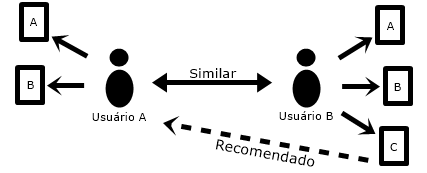
\includegraphics[scale = 0.35]{filtroutilizadoressimilares.png}

  \caption {Filtro Baseado em Utilizadores Similares}

  \label {fig01}

\end{figure}



\subsubsection{ Filtros Colaborativos Baseados em itens}
\par\hfill
 \par Para fazer previsões sobre se um utilizador A gostará de uma música B , o primeiro passo passa por determinar as X músicas mais semelhantes a B. As avaliações dadas por A a essas X músicas é usada para inferir se A gostará da música B.

 \par Este método é fácil de implementar, no entanto peca por falta de personalização.~\cite{ref_article1}.

\begin{figure}[H]

  \centering

  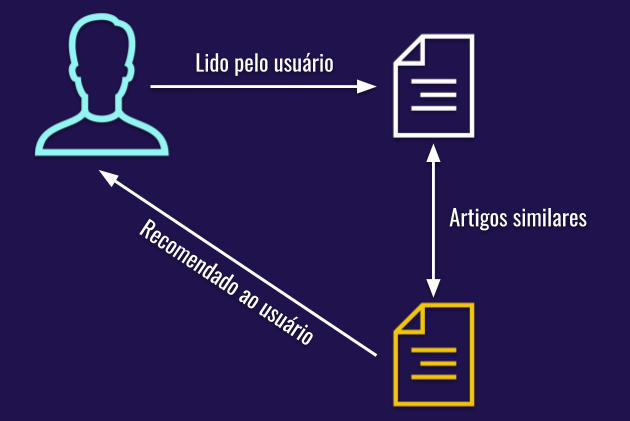
\includegraphics[scale = 0.2]{filtroitenssimilares.png}

  \caption{Filtro Baseado em itens Similares}

  \label{fig02}

\end{figure}
\par A vizinhança para estes métodos pode ser definida de duas formas:



\begin{center}
\normalsize{\bfseries Métodos Baseados em Memória}\hfill
\end{center}
\par\hfill
 \par Estes métodos são também conhecidos como algoritmos de filtros colaborativos de vizinhança. Nestes, as avaliações que um utilizador pode dar a certos itens é prevista com base na sua vizinhança.\newline


\begin{center}
\normalsize{\bfseries Métodos Baseados em Modelos}\hfill
\end{center}
\par\hfill
\par Nestes modelos, mineração de dados e aprendizagem máquina são usados no contexto de modelos de previsão.
\par Nos casos onde o modelo é parametrizado, os parâmetros são aprendidos dentro do contexto da otimização da "framework".


\subsection{Sistemas de Recomendação Baseados em Conteúdo}
\par\hfill
\par Nestes sistemas, os atributos descritivos dos itens são usados para fazer recomendações. O termo conteúdo refere-se às decrições dos itens. 
\par As classificações do utilizador, bem como os seus hábitos de compras são combinados com os atributos dos itens para fazer as recomendações. 
\par Por exemplo, num filme X o João atribuiu uma classificação elevada mas não temos acesso a mais nenhuma classificação do mesmo filme feita por outros utilizadores. Nestas situações Modelos de filtros colaborativos não servem. No entanto, a descrição do filme contém as mesmas palavras chave que outros filmes, logo estes podem ser sugeridos ao João.
\par Em métodos baseados em conteúdo as descrições dos itens, que estão marcadas com classificações são usadas para treino para criar sugestões específicas para o utilizador. Para cada utilizador os dados usados para treino do sistema de recomendação passam pelo histórico de compras e classificações.
\begin{figure}[H]
  \centering
    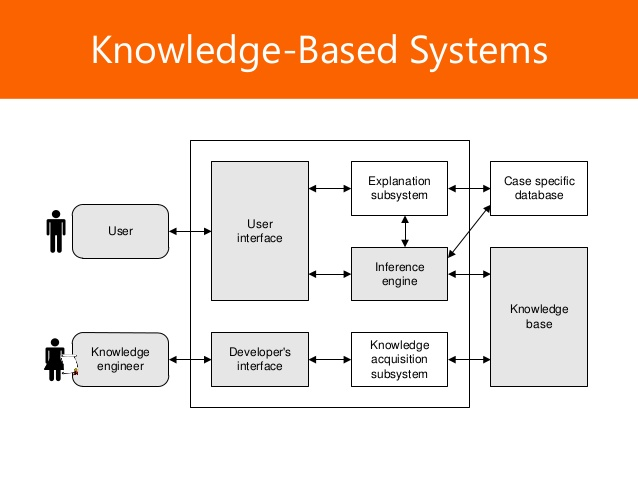
\includegraphics[scale = 0.3]{knoledgebasedsistems.jpeg}
    \caption{Sistema de Recomendação Baseado em Conteúdo}
    \label{fig03}
\end{figure}


\subsection{Sistemas de Recomendação Baseados em Conhecimento}
\par\hfill
\par Estes sistemas são particularmente úteis em casos em que não há histórico de compras ou avaliações, ou cenários de cold-start.
\par Para além disso, a natureza das preferências de um utilizador pode evoluir com o tempo. Como estes modelos utilizam as preferências dos itens conseguem acompanhar a tendência.
\par Em outros casos pode ser difícil acompanhar as preferências de um utilizador se este apenas estiver interessado num atributo específico do item.
\par O processo de escolha de recomendações baseia-se na similaridade entre requerimentos do utilizador e descrição dos itens, isto permite maior controlo do utilizador sobre o processo de recomendação podendo este explicitar o que pretende.
\par Estes sistemas podem ser classificados com base no tipo de interface: 
\hfill


\subsubsection{Sistemas de recomendação baseados em restrições}
\par\hfill
\par Utilizador especifica os atributos que pretende obter nos itens que procura. Regras específicas do domínio em que se insere a busca são utilizadas. Estas regras representam o conhecimento do sistema. Outras regras podem ser restrições no que diz respeito ao utilizador, por exemplo investidores experientes não fazem investimentos de alto risco. 
\par Posteriormente a uma pesquisa, o utilizador pode modificar os requisitos originais. Este processo é iterativo até o utilizador estar satisfeito com os resultados.



\subsubsection{Sistemas de recomendação baseados em casos}
\par\hfill
\par Neste tipo de sistemas, o utilizador especifica casos em vez de preferências como pontos de referência. As métricas de semelhança são cuidadosamente definidas no contexto do domínio em que se inserem, formando assim a base de conhecimento do sistema. Os resultados obtidos são comumente usados como referências para novas pesquisas do utilizador. Por exemplo, caso um resultado de pesquisa se assemelhe ao que o utilizador pretende, este pode selecionar esse resultado preferencial juntamente com alguns requerimentos extra na próxima pesquisa. Este processo guia o utilizador até ao item pretendido.
\par O sistema fornece sempre a oportunidade ao utilizador para mudar os requerimentos. No primeiro caso, as regras são usadas para guiar a busca com base nas similaridades com outros artigos. Já nos sistemas baseados em casos, o objeto de referência fornecido pelo utilizador é utilizado para calcular a similaridade com outros itens.
\par Os sistemas baseados em conhecimento partilham algumas das desvantagens
dos sistemas baseados em conteúdos, tendo como exemplo a falha de apresentar novo conteúdo que o utilizador não requisite, mas possa gostar. Para além disso, este sistema não aprende com o comportamento passado do utilizador, mas depende apenas dos requisitos que este inserir na pesquisa.



\subsubsection{Sistemas de recomendação baseados em utilidade}
\par\hfill
\par Sistemas que fazem uso de funções de utilidade para computar a probabilidade de um utilizador gostar do item em questão.
O desafio ao aplicar estes métodos reside em definir a função apropriada para o utilizador visado. Estas funções podem ser vistas como conhecimento externo, resultando na contemplação dos sistemas como casos específicos de sistemas de recomendação baseados em conhecimento, partilhando assim das suas vantagens e desvantagens.
\hfill

\subsection{Sistemas de Recomendação Demográficos}
\par\hfill
\par Nestas técnicas a localização do utilizador alvo é utilizada para saber a tendência de uma pessoa a comprar determinado produto. Por exemplo, nas zonas do país em que água é mais calcária que o normal, a tendência é de comprar detergentes que previnam o acumular deste mineral nas máquinas de lavar roupa.Em muitos casos, as informações demográficas podem ser combinadas com o contexto atual de informação do utilizador para guiar o proceso de recomendação.
\par Embora estes sistemas por si só não forneçam as melhores recomendações, combinados com outros sistemas produzem resultados significativamente melhores.


\subsection{Sistemas de Recomendação Híbridos/Agregados}
\par\hfill
 \par Nos três principais sistemas de recomendação descritos anteriormente, podemos observar que estes funcionam bem em cenários diferentes. 
 \par Os sistemas com filtros colaborativos dependem das avaliações da comunidade, métodos baseados em conteúdos dependem das descrições dos itens e avaliações do utilizador a quem a recomendação é feita e os sistemas baseados em conhecimento depende das interações sistema utilizador. Similarmente sistemas demográficos usam perfis demográficos para fazer recomendações.
 \par Como podemos observar cada uma das técnicas tem as suas vantagens e desvantagens, algumas funcionam melhor com cold-start e outras quando já têm uma base sólida de avaliações do utilizador. Isto leva-nos a concluir que, conjugando os vários sistemas, conseguimos construir algoritmos mais robustos e com melhor performance. Usualmente existe uma grande variedade de inputs o que nos dá a flexibilidade para empregar uma grande variedade de técnicas na mesma tarefa.
 \par Os sistemas híbridos estão extremamente relacionados com os campos da análise de conjuntos nos quais o poder de múltiplos tipos de algoritmo de aprendizagem máquina é combinado para criar um modelo mais robusto.
 \par Sistemas de recomendação agregados são capazes de combinar não só o poder de múltiplas fontes de dados como também ser altamente eficazes ao combinar múltiplos modelos num só tipo. Este cenário não é muito diferente da análise de conjuntos no campo de classificação de dados.

